\documentclass[1p]{elsarticle_modified}
%\bibliographystyle{elsarticle-num}

%\usepackage[colorlinks]{hyperref}
%\usepackage{abbrmath_seonhwa} %\Abb, \Ascr, \Acal ,\Abf, \Afrak
\usepackage{amsfonts}
\usepackage{amssymb}
\usepackage{amsmath}
\usepackage{amsthm}
\usepackage{scalefnt}
\usepackage{amsbsy}
\usepackage{kotex}
\usepackage{caption}
\usepackage{subfig}
\usepackage{color}
\usepackage{graphicx}
\usepackage{xcolor} %% white, black, red, green, blue, cyan, magenta, yellow
\usepackage{float}
\usepackage{setspace}
\usepackage{hyperref}

\usepackage{tikz}
\usetikzlibrary{arrows}

\usepackage{multirow}
\usepackage{array} % fixed length table
\usepackage{hhline}

%%%%%%%%%%%%%%%%%%%%%
\makeatletter
\renewcommand*\env@matrix[1][\arraystretch]{%
	\edef\arraystretch{#1}%
	\hskip -\arraycolsep
	\let\@ifnextchar\new@ifnextchar
	\array{*\c@MaxMatrixCols c}}
\makeatother %https://tex.stackexchange.com/questions/14071/how-can-i-increase-the-line-spacing-in-a-matrix
%%%%%%%%%%%%%%%

\usepackage[normalem]{ulem}

\newcommand{\msout}[1]{\ifmmode\text{\sout{\ensuremath{#1}}}\else\sout{#1}\fi}
%SOURCE: \msout is \stkout macro in https://tex.stackexchange.com/questions/20609/strikeout-in-math-mode

\newcommand{\cancel}[1]{
	\ifmmode
	{\color{red}\msout{#1}}
	\else
	{\color{red}\sout{#1}}
	\fi
}

\newcommand{\add}[1]{
	{\color{blue}\uwave{#1}}
}

\newcommand{\replace}[2]{
	\ifmmode
	{\color{red}\msout{#1}}{\color{blue}\uwave{#2}}
	\else
	{\color{red}\sout{#1}}{\color{blue}\uwave{#2}}
	\fi
}

\newcommand{\Sol}{\mathcal{S}} %segment
\newcommand{\D}{D} %diagram
\newcommand{\A}{\mathcal{A}} %arc


%%%%%%%%%%%%%%%%%%%%%%%%%%%%%5 test

\def\sl{\operatorname{\textup{SL}}(2,\Cbb)}
\def\psl{\operatorname{\textup{PSL}}(2,\Cbb)}
\def\quan{\mkern 1mu \triangleright \mkern 1mu}

\theoremstyle{definition}
\newtheorem{thm}{Theorem}[section]
\newtheorem{prop}[thm]{Proposition}
\newtheorem{lem}[thm]{Lemma}
\newtheorem{ques}[thm]{Question}
\newtheorem{cor}[thm]{Corollary}
\newtheorem{defn}[thm]{Definition}
\newtheorem{exam}[thm]{Example}
\newtheorem{rmk}[thm]{Remark}
\newtheorem{alg}[thm]{Algorithm}

\newcommand{\I}{\sqrt{-1}}
\begin{document}

%\begin{frontmatter}
%
%\title{Boundary parabolic representations of knots up to 8 crossings}
%
%%% Group authors per affiliation:
%\author{Yunhi Cho} 
%\address{Department of Mathematics, University of Seoul, Seoul, Korea}
%\ead{yhcho@uos.ac.kr}
%
%
%\author{Seonhwa Kim} %\fnref{s_kim}}
%\address{Center for Geometry and Physics, Institute for Basic Science, Pohang, 37673, Korea}
%\ead{ryeona17@ibs.re.kr}
%
%\author{Hyuk Kim}
%\address{Department of Mathematical Sciences, Seoul National University, Seoul 08826, Korea}
%\ead{hyukkim@snu.ac.kr}
%
%\author{Seokbeom Yoon}
%\address{Department of Mathematical Sciences, Seoul National University, Seoul, 08826,  Korea}
%\ead{sbyoon15@snu.ac.kr}
%
%\begin{abstract}
%We find all boundary parabolic representation of knots up to 8 crossings.
%
%\end{abstract}
%\begin{keyword}
%    \MSC[2010] 57M25 
%\end{keyword}
%
%\end{frontmatter}

%\linenumbers
%\tableofcontents
%
\newcommand\colored[1]{\textcolor{white}{\rule[-0.35ex]{0.8em}{1.4ex}}\kern-0.8em\color{red} #1}%
%\newcommand\colored[1]{\textcolor{white}{ #1}\kern-2.17ex	\textcolor{white}{ #1}\kern-1.81ex	\textcolor{white}{ #1}\kern-2.15ex\color{red}#1	}

{\Large $\underline{12n_{0801}~(K12n_{0801})}$}

\setlength{\tabcolsep}{10pt}
\renewcommand{\arraystretch}{1.6}
\vspace{1cm}\begin{tabular}{m{100pt}>{\centering\arraybackslash}m{274pt}}
\multirow{5}{120pt}{
	\centering
	\includegraphics[width=112pt]{../../../GIT/diagram.site/Diagrams/png/2890_12n_0801.png}\\
\ \ \ A knot diagram\footnotemark}&
\allowdisplaybreaks
\textbf{Linearized knot diagam} \\
\cline{2-2}
 &
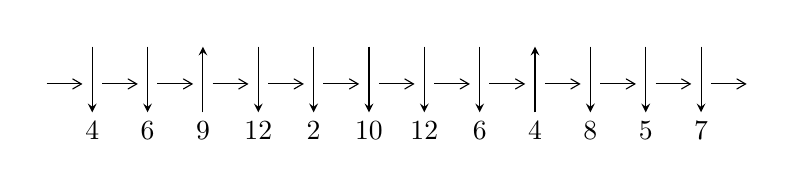
\begin{tikzpicture}[x=20pt, y=17pt]
	% nodes
	\node (C0) at (0, 0) {};
	\node (C1) at (1, 0) {};
	\node (C1U) at (1, +1) {};
	\node (C1D) at (1, -1) {4};

	\node (C2) at (2, 0) {};
	\node (C2U) at (2, +1) {};
	\node (C2D) at (2, -1) {6};

	\node (C3) at (3, 0) {};
	\node (C3U) at (3, +1) {};
	\node (C3D) at (3, -1) {9};

	\node (C4) at (4, 0) {};
	\node (C4U) at (4, +1) {};
	\node (C4D) at (4, -1) {12};

	\node (C5) at (5, 0) {};
	\node (C5U) at (5, +1) {};
	\node (C5D) at (5, -1) {2};

	\node (C6) at (6, 0) {};
	\node (C6U) at (6, +1) {};
	\node (C6D) at (6, -1) {10};

	\node (C7) at (7, 0) {};
	\node (C7U) at (7, +1) {};
	\node (C7D) at (7, -1) {12};

	\node (C8) at (8, 0) {};
	\node (C8U) at (8, +1) {};
	\node (C8D) at (8, -1) {6};

	\node (C9) at (9, 0) {};
	\node (C9U) at (9, +1) {};
	\node (C9D) at (9, -1) {4};

	\node (C10) at (10, 0) {};
	\node (C10U) at (10, +1) {};
	\node (C10D) at (10, -1) {8};

	\node (C11) at (11, 0) {};
	\node (C11U) at (11, +1) {};
	\node (C11D) at (11, -1) {5};

	\node (C12) at (12, 0) {};
	\node (C12U) at (12, +1) {};
	\node (C12D) at (12, -1) {7};
	\node (C13) at (13, 0) {};

	% arrows
	\draw[->,>={angle 60}]
	(C0) edge (C1) (C1) edge (C2) (C2) edge (C3) (C3) edge (C4) (C4) edge (C5) (C5) edge (C6) (C6) edge (C7) (C7) edge (C8) (C8) edge (C9) (C9) edge (C10) (C10) edge (C11) (C11) edge (C12) (C12) edge (C13) ;	\draw[->,>=stealth]
	(C1U) edge (C1D) (C2U) edge (C2D) (C3D) edge (C3U) (C4U) edge (C4D) (C5U) edge (C5D) (C6U) edge (C6D) (C7U) edge (C7D) (C8U) edge (C8D) (C9D) edge (C9U) (C10U) edge (C10D) (C11U) edge (C11D) (C12U) edge (C12D) ;
	\end{tikzpicture} \\
\hhline{~~} \\& 
\textbf{Solving Sequence} \\ \cline{2-2} 
 &
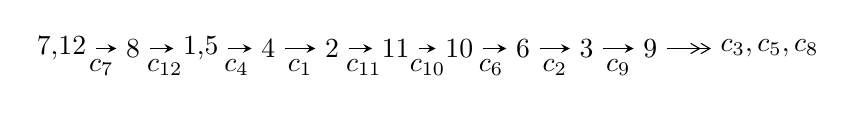
\begin{tikzpicture}[x=23pt, y=7pt]
	% node
	\node (A0) at (-1/8, 0) {7,12};
	\node (A1) at (1, 0) {8};
	\node (A2) at (33/16, 0) {1,5};
	\node (A3) at (25/8, 0) {4};
	\node (A4) at (33/8, 0) {2};
	\node (A5) at (41/8, 0) {11};
	\node (A6) at (49/8, 0) {10};
	\node (A7) at (57/8, 0) {6};
	\node (A8) at (65/8, 0) {3};
	\node (A9) at (73/8, 0) {9};
	\node (C1) at (1/2, -1) {$c_{7}$};
	\node (C2) at (3/2, -1) {$c_{12}$};
	\node (C3) at (21/8, -1) {$c_{4}$};
	\node (C4) at (29/8, -1) {$c_{1}$};
	\node (C5) at (37/8, -1) {$c_{11}$};
	\node (C6) at (45/8, -1) {$c_{10}$};
	\node (C7) at (53/8, -1) {$c_{6}$};
	\node (C8) at (61/8, -1) {$c_{2}$};
	\node (C9) at (69/8, -1) {$c_{9}$};
	\node (A10) at (11, 0) {$c_{3},c_{5},c_{8}$};

	% edge
	\draw[->,>=stealth]	
	(A0) edge (A1) (A1) edge (A2) (A2) edge (A3) (A3) edge (A4) (A4) edge (A5) (A5) edge (A6) (A6) edge (A7) (A7) edge (A8) (A8) edge (A9) ;
	\draw[->>,>={angle 60}]	
	(A9) edge (A10);
\end{tikzpicture} \\ 

\end{tabular} \\

\footnotetext{
The image of knot diagram is generated by the software ``\textbf{Draw programme}" developed by Andrew Bartholomew(\url{http://www.layer8.co.uk/maths/draw/index.htm\#Running-draw}), where we modified some parts for our purpose(\url{https://github.com/CATsTAILs/LinksPainter}).
}\phantom \\ \newline 
\centering \textbf{Ideals for irreducible components\footnotemark of $X_{\text{par}}$} 
 
\begin{align*}
I^u_{1}&=\langle 
139726521 u^{15}-216650645 u^{14}+\cdots+864519475 b-245546684,\;a-1,\;u^{16}- u^{15}+\cdots-3 u^2-1\rangle \\
I^u_{2}&=\langle 
- u^6+u^5- u^4+10 u^3+13 u^2+5 b+u+1,\;a+1,\;u^7+5 u^5-4 u^4+7 u^3-4 u^2+3 u-1\rangle \\
I^u_{3}&=\langle 
-51 u^{11}-95 u^{10}+\cdots+185 b+342,\;-224 u^{11}-188 u^{10}+\cdots+185 a-115,\\
\phantom{I^u_{3}}&\phantom{= \langle  }u^{12}+u^{11}+5 u^{10}+5 u^9+9 u^8+6 u^7+u^6-5 u^5-11 u^4-15 u^3-11 u^2-4 u-1\rangle \\
I^u_{4}&=\langle 
-964489278415 u^{11}+117148284431 u^{10}+\cdots+301017906283623 b+191146639374112,\\
\phantom{I^u_{4}}&\phantom{= \langle  }199776571521368 u^{11}-160244377858182 u^{10}+\cdots+8729519282225067 a-77902584840567367,\\
\phantom{I^u_{4}}&\phantom{= \langle  }u^{12}- u^{11}+15 u^{10}-3 u^9+83 u^8+74 u^7+245 u^6+355 u^5+477 u^4+227 u^3-109 u^2-372 u+29\rangle \\
\\
\end{align*}
\raggedright * 4 irreducible components of $\dim_{\mathbb{C}}=0$, with total 47 representations.\\
\footnotetext{All coefficients of polynomials are rational numbers. But the coefficients are sometimes approximated in decimal forms when there is not enough margin.}
\newpage
\renewcommand{\arraystretch}{1}
\centering \section*{I. $I^u_{1}= \langle 1.40\times10^{8} u^{15}-2.17\times10^{8} u^{14}+\cdots+8.65\times10^{8} b-2.46\times10^{8},\;a-1,\;u^{16}- u^{15}+\cdots-3 u^2-1 \rangle$}
\flushleft \textbf{(i) Arc colorings}\\
\begin{tabular}{m{7pt} m{180pt} m{7pt} m{180pt} }
\flushright $a_{7}=$&$\begin{pmatrix}1\\0\end{pmatrix}$ \\
\flushright $a_{12}=$&$\begin{pmatrix}0\\u\end{pmatrix}$ \\
\flushright $a_{8}=$&$\begin{pmatrix}1\\u^2\end{pmatrix}$ \\
\flushright $a_{1}=$&$\begin{pmatrix}- u\\u\end{pmatrix}$ \\
\flushright $a_{5}=$&$\begin{pmatrix}1\\-0.161623 u^{15}+0.250602 u^{14}+\cdots-0.962108 u+0.284027\end{pmatrix}$ \\
\flushright $a_{4}=$&$\begin{pmatrix}1\\-0.161623 u^{15}+0.250602 u^{14}+\cdots-0.962108 u+0.284027\end{pmatrix}$ \\
\flushright $a_{2}=$&$\begin{pmatrix}-0.0889791 u^{15}+0.0677199 u^{14}+\cdots-2.28403 u+0.161623\\-0.457683 u^{15}+0.568849 u^{14}+\cdots+0.832397 u+0.604244\end{pmatrix}$ \\
\flushright $a_{11}=$&$\begin{pmatrix}u\\0.0889791 u^{15}-0.0677199 u^{14}+\cdots+1.28403 u-0.161623\end{pmatrix}$ \\
\flushright $a_{10}=$&$\begin{pmatrix}0.0889791 u^{15}-0.0677199 u^{14}+\cdots+2.28403 u-0.161623\\0.158988 u^{15}-0.177074 u^{14}+\cdots+1.37301 u-0.140364\end{pmatrix}$ \\
\flushright $a_{6}=$&$\begin{pmatrix}0.127953 u^{15}+0.0697779 u^{14}+\cdots+0.974879 u+0.182022\\-0.145027 u^{15}+0.362922 u^{14}+\cdots+0.962468 u-0.461260\end{pmatrix}$ \\
\flushright $a_{3}=$&$\begin{pmatrix}-0.831219 u^{15}+0.864475 u^{14}+\cdots-2.13140 u+0.842638\\-0.913992 u^{15}+1.16510 u^{14}+\cdots+1.31352 u+1.03630\end{pmatrix}$ \\
\flushright $a_{9}=$&$\begin{pmatrix}0.476653 u^{15}-0.527214 u^{14}+\cdots+1.36265 u-0.787127\\0.687117 u^{15}-0.912956 u^{14}+\cdots+0.517385 u-0.960091\end{pmatrix}$\\&\end{tabular}
\flushleft \textbf{(ii) Obstruction class $= -1$}\\~\\
\flushleft \textbf{(iii) Cusp Shapes $= -\frac{447574308}{864519475} u^{15}-\frac{223753298}{172903895} u^{14}+\cdots+\frac{6627598422}{864519475} u-\frac{4377348818}{864519475}$}\\~\\
\newpage\renewcommand{\arraystretch}{1}
\flushleft \textbf{(iv) u-Polynomials at the component}\newline \\
\begin{tabular}{m{50pt}|m{274pt}}
Crossings & \hspace{64pt}u-Polynomials at each crossing \\
\hline $$\begin{aligned}c_{1},c_{10}\end{aligned}$$&$\begin{aligned}
&u^{16}-2 u^{15}+\cdots-63 u-27
\end{aligned}$\\
\hline $$\begin{aligned}c_{2},c_{5},c_{6}\end{aligned}$$&$\begin{aligned}
&u^{16}+2 u^{15}+\cdots+14 u+1
\end{aligned}$\\
\hline $$\begin{aligned}c_{3},c_{9}\end{aligned}$$&$\begin{aligned}
&u^{16}+7 u^{15}+\cdots+39 u+19
\end{aligned}$\\
\hline $$\begin{aligned}c_{4},c_{7},c_{11}\\c_{12}\end{aligned}$$&$\begin{aligned}
&u^{16}+u^{15}+\cdots-3 u^2-1
\end{aligned}$\\
\hline $$\begin{aligned}c_{8}\end{aligned}$$&$\begin{aligned}
&u^{16}+2 u^{15}+\cdots+4 u+1
\end{aligned}$\\
\hline
\end{tabular}\\~\\
\newpage\renewcommand{\arraystretch}{1}
\flushleft \textbf{(v) Riley Polynomials at the component}\newline \\
\begin{tabular}{m{50pt}|m{274pt}}
Crossings & \hspace{64pt}Riley Polynomials at each crossing \\
\hline $$\begin{aligned}c_{1},c_{10}\end{aligned}$$&$\begin{aligned}
&y^{16}+36 y^{15}+\cdots-4131 y+729
\end{aligned}$\\
\hline $$\begin{aligned}c_{2},c_{5},c_{6}\end{aligned}$$&$\begin{aligned}
&y^{16}+4 y^{15}+\cdots-104 y+1
\end{aligned}$\\
\hline $$\begin{aligned}c_{3},c_{9}\end{aligned}$$&$\begin{aligned}
&y^{16}-17 y^{15}+\cdots-1977 y+361
\end{aligned}$\\
\hline $$\begin{aligned}c_{4},c_{7},c_{11}\\c_{12}\end{aligned}$$&$\begin{aligned}
&y^{16}+21 y^{15}+\cdots+6 y+1
\end{aligned}$\\
\hline $$\begin{aligned}c_{8}\end{aligned}$$&$\begin{aligned}
&y^{16}+16 y^{15}+\cdots+8 y+1
\end{aligned}$\\
\hline
\end{tabular}\\~\\
\newpage\flushleft \textbf{(vi) Complex Volumes and Cusp Shapes}
$$\begin{array}{c|c|c}  
\text{Solutions to }I^u_{1}& \I (\text{vol} + \sqrt{-1}CS) & \text{Cusp shape}\\
 \hline 
\begin{aligned}
u &= \phantom{-}0.315992 + 0.923692 I \\
a &= \phantom{-}1.00000\phantom{ +0.000000I} \\
b &= -1.072170 + 0.739909 I\end{aligned}
 & \phantom{-}0.73896 - 4.05435 I & -4.39569 + 8.69732 I \\ \hline\begin{aligned}
u &= \phantom{-}0.315992 - 0.923692 I \\
a &= \phantom{-}1.00000\phantom{ +0.000000I} \\
b &= -1.072170 - 0.739909 I\end{aligned}
 & \phantom{-}0.73896 + 4.05435 I & -4.39569 - 8.69732 I \\ \hline\begin{aligned}
u &= -0.946702\phantom{ +0.000000I} \\
a &= \phantom{-}1.00000\phantom{ +0.000000I} \\
b &= -0.982882\phantom{ +0.000000I}\end{aligned}
 & -3.88612\phantom{ +0.000000I} & -24.3560\phantom{ +0.000000I} \\ \hline\begin{aligned}
u &= -0.012719 + 1.092980 I \\
a &= \phantom{-}1.00000\phantom{ +0.000000I} \\
b &= -1.42699 + 0.92099 I\end{aligned}
 & \phantom{-}10.45990 + 3.54053 I & \phantom{-}0.82342 - 2.71051 I \\ \hline\begin{aligned}
u &= -0.012719 - 1.092980 I \\
a &= \phantom{-}1.00000\phantom{ +0.000000I} \\
b &= -1.42699 - 0.92099 I\end{aligned}
 & \phantom{-}10.45990 - 3.54053 I & \phantom{-}0.82342 + 2.71051 I \\ \hline\begin{aligned}
u &= -0.212701 + 0.840300 I \\
a &= \phantom{-}1.00000\phantom{ +0.000000I} \\
b &= -1.02555 - 1.53512 I\end{aligned}
 & -0.301618 + 0.879889 I & -7.11415 - 1.14520 I \\ \hline\begin{aligned}
u &= -0.212701 - 0.840300 I \\
a &= \phantom{-}1.00000\phantom{ +0.000000I} \\
b &= -1.02555 + 1.53512 I\end{aligned}
 & -0.301618 - 0.879889 I & -7.11415 + 1.14520 I \\ \hline\begin{aligned}
u &= \phantom{-}1.24735\phantom{ +0.000000I} \\
a &= \phantom{-}1.00000\phantom{ +0.000000I} \\
b &= -0.0213320\phantom{ +0.000000I}\end{aligned}
 & -2.33062\phantom{ +0.000000I} & -0.734580\phantom{ +0.000000I} \\ \hline\begin{aligned}
u &= -0.361980 + 0.330445 I \\
a &= \phantom{-}1.00000\phantom{ +0.000000I} \\
b &= \phantom{-}1.42983 + 0.27839 I\end{aligned}
 & \phantom{-}5.02983 + 5.57711 I & -7.96481 - 3.29725 I \\ \hline\begin{aligned}
u &= -0.361980 - 0.330445 I \\
a &= \phantom{-}1.00000\phantom{ +0.000000I} \\
b &= \phantom{-}1.42983 - 0.27839 I\end{aligned}
 & \phantom{-}5.02983 - 5.57711 I & -7.96481 + 3.29725 I\\
 \hline 
 \end{array}$$\newpage$$\begin{array}{c|c|c}  
\text{Solutions to }I^u_{1}& \I (\text{vol} + \sqrt{-1}CS) & \text{Cusp shape}\\
 \hline 
\begin{aligned}
u &= \phantom{-}0.264024 + 0.315325 I \\
a &= \phantom{-}1.00000\phantom{ +0.000000I} \\
b &= \phantom{-}0.055251 - 0.498554 I\end{aligned}
 & -0.654553 - 0.896356 I & -9.07271 + 7.71736 I \\ \hline\begin{aligned}
u &= \phantom{-}0.264024 - 0.315325 I \\
a &= \phantom{-}1.00000\phantom{ +0.000000I} \\
b &= \phantom{-}0.055251 + 0.498554 I\end{aligned}
 & -0.654553 + 0.896356 I & -9.07271 - 7.71736 I \\ \hline\begin{aligned}
u &= -0.28076 + 1.98483 I \\
a &= \phantom{-}1.00000\phantom{ +0.000000I} \\
b &= -6.38980 - 0.96015 I\end{aligned}
 & \phantom{-}15.0967 + 4.8816 I & -2.19849 - 4.64135 I \\ \hline\begin{aligned}
u &= -0.28076 - 1.98483 I \\
a &= \phantom{-}1.00000\phantom{ +0.000000I} \\
b &= -6.38980 + 0.96015 I\end{aligned}
 & \phantom{-}15.0967 - 4.8816 I & -2.19849 + 4.64135 I \\ \hline\begin{aligned}
u &= \phantom{-}0.63782 + 2.37815 I \\
a &= \phantom{-}1.00000\phantom{ +0.000000I} \\
b &= -7.56846 + 2.89468 I\end{aligned}
 & -14.9238 - 11.4240 I & -3.53223 + 3.90898 I \\ \hline\begin{aligned}
u &= \phantom{-}0.63782 - 2.37815 I \\
a &= \phantom{-}1.00000\phantom{ +0.000000I} \\
b &= -7.56846 - 2.89468 I\end{aligned}
 & -14.9238 + 11.4240 I & -3.53223 - 3.90898 I\\
 \hline 
 \end{array}$$\newpage\newpage\renewcommand{\arraystretch}{1}
\centering \section*{II. $I^u_{2}= \langle - u^6+u^5- u^4+10 u^3+13 u^2+5 b+u+1,\;a+1,\;u^7+5 u^5-4 u^4+7 u^3-4 u^2+3 u-1 \rangle$}
\flushleft \textbf{(i) Arc colorings}\\
\begin{tabular}{m{7pt} m{180pt} m{7pt} m{180pt} }
\flushright $a_{7}=$&$\begin{pmatrix}1\\0\end{pmatrix}$ \\
\flushright $a_{12}=$&$\begin{pmatrix}0\\u\end{pmatrix}$ \\
\flushright $a_{8}=$&$\begin{pmatrix}1\\u^2\end{pmatrix}$ \\
\flushright $a_{1}=$&$\begin{pmatrix}- u\\u\end{pmatrix}$ \\
\flushright $a_{5}=$&$\begin{pmatrix}-1\\\frac{1}{5} u^6-\frac{1}{5} u^5+\cdots-\frac{1}{5} u-\frac{1}{5}\end{pmatrix}$ \\
\flushright $a_{4}=$&$\begin{pmatrix}-1\\\frac{1}{5} u^6-\frac{1}{5} u^5+\cdots-\frac{1}{5} u-\frac{1}{5}\end{pmatrix}$ \\
\flushright $a_{2}=$&$\begin{pmatrix}-\frac{1}{5} u^6-\frac{4}{5} u^5+\cdots-\frac{14}{5} u+\frac{1}{5}\\u^5+5 u^3-3 u^2+5 u-2\end{pmatrix}$ \\
\flushright $a_{11}=$&$\begin{pmatrix}u\\\frac{1}{5} u^6+\frac{4}{5} u^5+\cdots+\frac{9}{5} u-\frac{1}{5}\end{pmatrix}$ \\
\flushright $a_{10}=$&$\begin{pmatrix}\frac{1}{5} u^6+\frac{4}{5} u^5+\cdots+\frac{14}{5} u-\frac{1}{5}\\\frac{2}{5} u^6+\frac{3}{5} u^5+\cdots-\frac{2}{5} u+\frac{3}{5}\end{pmatrix}$ \\
\flushright $a_{6}=$&$\begin{pmatrix}0\\\frac{3}{5} u^6+\frac{2}{5} u^5+\cdots-\frac{3}{5} u-\frac{3}{5}\end{pmatrix}$ \\
\flushright $a_{3}=$&$\begin{pmatrix}-\frac{1}{5} u^6-\frac{4}{5} u^5+\cdots-\frac{14}{5} u+\frac{1}{5}\\-\frac{6}{5} u^6+\frac{6}{5} u^5+\cdots+\frac{46}{5} u-\frac{19}{5}\end{pmatrix}$ \\
\flushright $a_{9}=$&$\begin{pmatrix}1\\u^5+u^4+5 u^3+u^2+3 u-1\end{pmatrix}$\\&\end{tabular}
\flushleft \textbf{(ii) Obstruction class $= 1$}\\~\\
\flushleft \textbf{(iii) Cusp Shapes $= -\frac{43}{5} u^6-\frac{12}{5} u^5-\frac{208}{5} u^4+24 u^3-\frac{216}{5} u^2+\frac{93}{5} u-\frac{82}{5}$}\\~\\
\newpage\renewcommand{\arraystretch}{1}
\flushleft \textbf{(iv) u-Polynomials at the component}\newline \\
\begin{tabular}{m{50pt}|m{274pt}}
Crossings & \hspace{64pt}u-Polynomials at each crossing \\
\hline $$\begin{aligned}c_{1}\end{aligned}$$&$\begin{aligned}
&u^7- u^6+7 u^5-3 u^4-13 u^3+7 u^2+8 u-5
\end{aligned}$\\
\hline $$\begin{aligned}c_{2},c_{6}\end{aligned}$$&$\begin{aligned}
&u^7+u^6+u^5- u^4- u^2+u-1
\end{aligned}$\\
\hline $$\begin{aligned}c_{3}\end{aligned}$$&$\begin{aligned}
&u^7-6 u^6+16 u^5-25 u^4+26 u^3-18 u^2+6 u+1
\end{aligned}$\\
\hline $$\begin{aligned}c_{4},c_{12}\end{aligned}$$&$\begin{aligned}
&u^7+5 u^5+4 u^4+7 u^3+4 u^2+3 u+1
\end{aligned}$\\
\hline $$\begin{aligned}c_{5}\end{aligned}$$&$\begin{aligned}
&u^7- u^6+u^5+u^4+u^2+u+1
\end{aligned}$\\
\hline $$\begin{aligned}c_{7},c_{11}\end{aligned}$$&$\begin{aligned}
&u^7+5 u^5-4 u^4+7 u^3-4 u^2+3 u-1
\end{aligned}$\\
\hline $$\begin{aligned}c_{8}\end{aligned}$$&$\begin{aligned}
&u^7- u^6+3 u^5-3 u^4+2 u^3+3 u^2- u+1
\end{aligned}$\\
\hline $$\begin{aligned}c_{9}\end{aligned}$$&$\begin{aligned}
&u^7+6 u^6+16 u^5+25 u^4+26 u^3+18 u^2+6 u-1
\end{aligned}$\\
\hline $$\begin{aligned}c_{10}\end{aligned}$$&$\begin{aligned}
&u^7+u^6+7 u^5+3 u^4-13 u^3-7 u^2+8 u+5
\end{aligned}$\\
\hline
\end{tabular}\\~\\
\newpage\renewcommand{\arraystretch}{1}
\flushleft \textbf{(v) Riley Polynomials at the component}\newline \\
\begin{tabular}{m{50pt}|m{274pt}}
Crossings & \hspace{64pt}Riley Polynomials at each crossing \\
\hline $$\begin{aligned}c_{1},c_{10}\end{aligned}$$&$\begin{aligned}
&y^7+13 y^6+17 y^5-161 y^4+313 y^3-287 y^2+134 y-25
\end{aligned}$\\
\hline $$\begin{aligned}c_{2},c_{5},c_{6}\end{aligned}$$&$\begin{aligned}
&y^7+y^6+3 y^5+3 y^4+2 y^3-3 y^2- y-1
\end{aligned}$\\
\hline $$\begin{aligned}c_{3},c_{9}\end{aligned}$$&$\begin{aligned}
&y^7-4 y^6+8 y^5+3 y^4-20 y^3+38 y^2+72 y-1
\end{aligned}$\\
\hline $$\begin{aligned}c_{4},c_{7},c_{11}\\c_{12}\end{aligned}$$&$\begin{aligned}
&y^7+10 y^6+39 y^5+60 y^4+47 y^3+18 y^2+y-1
\end{aligned}$\\
\hline $$\begin{aligned}c_{8}\end{aligned}$$&$\begin{aligned}
&y^7+5 y^6+7 y^5+7 y^4+18 y^3-7 y^2-5 y-1
\end{aligned}$\\
\hline
\end{tabular}\\~\\
\newpage\flushleft \textbf{(vi) Complex Volumes and Cusp Shapes}
$$\begin{array}{c|c|c}  
\text{Solutions to }I^u_{2}& \I (\text{vol} + \sqrt{-1}CS) & \text{Cusp shape}\\
 \hline 
\begin{aligned}
u &= \phantom{-}0.381257 + 0.787604 I \\
a &= -1.00000\phantom{ +0.000000I} \\
b &= \phantom{-}2.24160 - 1.44010 I\end{aligned}
 & \phantom{-}5.73082 - 6.35876 I & -3.32185 + 8.09951 I \\ \hline\begin{aligned}
u &= \phantom{-}0.381257 - 0.787604 I \\
a &= -1.00000\phantom{ +0.000000I} \\
b &= \phantom{-}2.24160 + 1.44010 I\end{aligned}
 & \phantom{-}5.73082 + 6.35876 I & -3.32185 - 8.09951 I \\ \hline\begin{aligned}
u &= -0.060693 + 0.837302 I \\
a &= -1.00000\phantom{ +0.000000I} \\
b &= \phantom{-}1.43171 + 1.17322 I\end{aligned}
 & \phantom{-}0.771836 + 0.196666 I & -1.060679 + 0.531434 I \\ \hline\begin{aligned}
u &= -0.060693 - 0.837302 I \\
a &= -1.00000\phantom{ +0.000000I} \\
b &= \phantom{-}1.43171 - 1.17322 I\end{aligned}
 & \phantom{-}0.771836 - 0.196666 I & -1.060679 - 0.531434 I \\ \hline\begin{aligned}
u &= \phantom{-}0.414510\phantom{ +0.000000I} \\
a &= -1.00000\phantom{ +0.000000I} \\
b &= -0.867599\phantom{ +0.000000I}\end{aligned}
 & -2.57196\phantom{ +0.000000I} & -15.7040\phantom{ +0.000000I} \\ \hline\begin{aligned}
u &= -0.52782 + 2.04747 I \\
a &= -1.00000\phantom{ +0.000000I} \\
b &= \phantom{-}6.26049 + 1.92207 I\end{aligned}
 & \phantom{-}14.5225 + 3.4415 I & -3.76523 - 0.87607 I \\ \hline\begin{aligned}
u &= -0.52782 - 2.04747 I \\
a &= -1.00000\phantom{ +0.000000I} \\
b &= \phantom{-}6.26049 - 1.92207 I\end{aligned}
 & \phantom{-}14.5225 - 3.4415 I & -3.76523 + 0.87607 I\\
 \hline 
 \end{array}$$\newpage\newpage\renewcommand{\arraystretch}{1}
\centering \section*{III. $I^u_{3}= \langle -51 u^{11}-95 u^{10}+\cdots+185 b+342,\;-224 u^{11}-188 u^{10}+\cdots+185 a-115,\;u^{12}+u^{11}+\cdots-4 u-1 \rangle$}
\flushleft \textbf{(i) Arc colorings}\\
\begin{tabular}{m{7pt} m{180pt} m{7pt} m{180pt} }
\flushright $a_{7}=$&$\begin{pmatrix}1\\0\end{pmatrix}$ \\
\flushright $a_{12}=$&$\begin{pmatrix}0\\u\end{pmatrix}$ \\
\flushright $a_{8}=$&$\begin{pmatrix}1\\u^2\end{pmatrix}$ \\
\flushright $a_{1}=$&$\begin{pmatrix}- u\\u\end{pmatrix}$ \\
\flushright $a_{5}=$&$\begin{pmatrix}1.21081 u^{11}+1.01622 u^{10}+\cdots-6.87027 u+0.621622\\0.275676 u^{11}+0.513514 u^{10}+\cdots-4.89189 u-1.84865\end{pmatrix}$ \\
\flushright $a_{4}=$&$\begin{pmatrix}1.21081 u^{11}+1.01622 u^{10}+\cdots-6.87027 u+0.621622\\0.772973 u^{11}+0.459459 u^{10}+\cdots-5.32432 u-1.65405\end{pmatrix}$ \\
\flushright $a_{2}=$&$\begin{pmatrix}1.88108 u^{11}+2.02162 u^{10}+\cdots-20.8270 u-6.03784\\-0.832432 u^{11}-0.448649 u^{10}+\cdots+4.41081 u+0.135135\end{pmatrix}$ \\
\flushright $a_{11}=$&$\begin{pmatrix}-2.07027 u^{11}-2.20541 u^{10}+\cdots+20.3568 u+5.25946\\0.821622 u^{11}+0.232432 u^{10}+\cdots-2.14054 u+0.643243\end{pmatrix}$ \\
\flushright $a_{10}=$&$\begin{pmatrix}-1.88108 u^{11}-2.02162 u^{10}+\cdots+20.8270 u+6.03784\\0.518919 u^{11}+0.378378 u^{10}+\cdots-1.97297 u+0.637838\end{pmatrix}$ \\
\flushright $a_{6}=$&$\begin{pmatrix}1.46486 u^{11}+2.49730 u^{10}+\cdots-24.0216 u-6.27027\\-0.637838 u^{11}-0.356757 u^{10}+\cdots+3.14595 u-0.675676\end{pmatrix}$ \\
\flushright $a_{3}=$&$\begin{pmatrix}0.627027 u^{11}-1.05946 u^{10}+\cdots+7.52432 u+4.25405\\0.432432 u^{11}+0.448649 u^{10}+\cdots-3.41081 u-0.335135\end{pmatrix}$ \\
\flushright $a_{9}=$&$\begin{pmatrix}-2.70811 u^{11}-2.16216 u^{10}+\cdots+23.7027 u+4.98378\\0.329730 u^{11}-0.00540541 u^{10}+\cdots+0.956757 u+1.65946\end{pmatrix}$\\&\end{tabular}
\flushleft \textbf{(ii) Obstruction class $= 1$}\\~\\
\flushleft \textbf{(iii) Cusp Shapes $= \frac{117}{185} u^{11}+\frac{24}{37} u^{10}+\frac{608}{185} u^9+\frac{593}{185} u^8+\frac{1109}{185} u^7+\frac{683}{185} u^6+\frac{14}{37} u^5-\frac{661}{185} u^4-\frac{1488}{185} u^3-\frac{337}{37} u^2-\frac{252}{37} u-\frac{1024}{185}$}\\~\\
\newpage\renewcommand{\arraystretch}{1}
\flushleft \textbf{(iv) u-Polynomials at the component}\newline \\
\begin{tabular}{m{50pt}|m{274pt}}
Crossings & \hspace{64pt}u-Polynomials at each crossing \\
\hline $$\begin{aligned}c_{1}\end{aligned}$$&$\begin{aligned}
&u^{12}+4 u^{11}+\cdots-20 u-5
\end{aligned}$\\
\hline $$\begin{aligned}c_{2},c_{6}\end{aligned}$$&$\begin{aligned}
&u^{12}+2 u^{11}+\cdots-5 u+1
\end{aligned}$\\
\hline $$\begin{aligned}c_{3}\end{aligned}$$&$\begin{aligned}
&(u^2+u-1)^6
\end{aligned}$\\
\hline $$\begin{aligned}c_{4},c_{12}\end{aligned}$$&$\begin{aligned}
&u^{12}- u^{11}+\cdots+4 u-1
\end{aligned}$\\
\hline $$\begin{aligned}c_{5}\end{aligned}$$&$\begin{aligned}
&u^{12}-2 u^{11}+\cdots+5 u+1
\end{aligned}$\\
\hline $$\begin{aligned}c_{7},c_{11}\end{aligned}$$&$\begin{aligned}
&u^{12}+u^{11}+\cdots-4 u-1
\end{aligned}$\\
\hline $$\begin{aligned}c_{8}\end{aligned}$$&$\begin{aligned}
&u^{12}+2 u^{11}+\cdots+25 u+25
\end{aligned}$\\
\hline $$\begin{aligned}c_{9}\end{aligned}$$&$\begin{aligned}
&(u^2- u-1)^6
\end{aligned}$\\
\hline $$\begin{aligned}c_{10}\end{aligned}$$&$\begin{aligned}
&u^{12}-4 u^{11}+\cdots+20 u-5
\end{aligned}$\\
\hline
\end{tabular}\\~\\
\newpage\renewcommand{\arraystretch}{1}
\flushleft \textbf{(v) Riley Polynomials at the component}\newline \\
\begin{tabular}{m{50pt}|m{274pt}}
Crossings & \hspace{64pt}Riley Polynomials at each crossing \\
\hline $$\begin{aligned}c_{1},c_{10}\end{aligned}$$&$\begin{aligned}
&y^{12}-2 y^{11}+\cdots-550 y+25
\end{aligned}$\\
\hline $$\begin{aligned}c_{2},c_{5},c_{6}\end{aligned}$$&$\begin{aligned}
&y^{12}-4 y^{11}+\cdots-49 y+1
\end{aligned}$\\
\hline $$\begin{aligned}c_{3},c_{9}\end{aligned}$$&$\begin{aligned}
&(y^2-3 y+1)^6
\end{aligned}$\\
\hline $$\begin{aligned}c_{4},c_{7},c_{11}\\c_{12}\end{aligned}$$&$\begin{aligned}
&y^{12}+9 y^{11}+\cdots+6 y+1
\end{aligned}$\\
\hline $$\begin{aligned}c_{8}\end{aligned}$$&$\begin{aligned}
&y^{12}+8 y^{11}+\cdots-125 y+625
\end{aligned}$\\
\hline
\end{tabular}\\~\\
\newpage\flushleft \textbf{(vi) Complex Volumes and Cusp Shapes}
$$\begin{array}{c|c|c}  
\text{Solutions to }I^u_{3}& \I (\text{vol} + \sqrt{-1}CS) & \text{Cusp shape}\\
 \hline 
\begin{aligned}
u &= \phantom{-}1.09790\phantom{ +0.000000I} \\
a &= \phantom{-}0.679223\phantom{ +0.000000I} \\
b &= -0.936157\phantom{ +0.000000I}\end{aligned}
 & -3.41636\phantom{ +0.000000I} & -3.43020\phantom{ +0.000000I} \\ \hline\begin{aligned}
u &= -0.686696 + 0.529141 I \\
a &= -0.80710 + 1.68749 I \\
b &= \phantom{-}0.949158 + 0.164926 I\end{aligned}
 & \phantom{-}8.61690 + 2.82812 I & -3.78492 - 1.30714 I \\ \hline\begin{aligned}
u &= -0.686696 - 0.529141 I \\
a &= -0.80710 - 1.68749 I \\
b &= \phantom{-}0.949158 - 0.164926 I\end{aligned}
 & \phantom{-}8.61690 - 2.82812 I & -3.78492 + 1.30714 I \\ \hline\begin{aligned}
u &= \phantom{-}0.318837 + 1.198780 I \\
a &= \phantom{-}0.343080 - 0.063834 I \\
b &= -0.531922 + 1.092370 I\end{aligned}
 & \phantom{-}0.72122 - 2.82812 I & -3.78492 + 1.30714 I \\ \hline\begin{aligned}
u &= \phantom{-}0.318837 - 1.198780 I \\
a &= \phantom{-}0.343080 + 0.063834 I \\
b &= -0.531922 - 1.092370 I\end{aligned}
 & \phantom{-}0.72122 + 2.82812 I & -3.78492 - 1.30714 I \\ \hline\begin{aligned}
u &= -0.745717\phantom{ +0.000000I} \\
a &= \phantom{-}1.47227\phantom{ +0.000000I} \\
b &= -0.936157\phantom{ +0.000000I}\end{aligned}
 & -3.41636\phantom{ +0.000000I} & -3.43020\phantom{ +0.000000I} \\ \hline\begin{aligned}
u &= -0.46101 + 1.38957 I \\
a &= \phantom{-}0.801692 - 0.597738 I \\
b &= -3.89832\phantom{ +0.000000I}\end{aligned}
 & \phantom{-}4.47932\phantom{ +0.000000I} & -3.43016 + 0. I\phantom{ +0.000000I} \\ \hline\begin{aligned}
u &= -0.46101 - 1.38957 I \\
a &= \phantom{-}0.801692 + 0.597738 I \\
b &= -3.89832\phantom{ +0.000000I}\end{aligned}
 & \phantom{-}4.47932\phantom{ +0.000000I} & -3.43016 + 0. I\phantom{ +0.000000I} \\ \hline\begin{aligned}
u &= -0.185910 + 0.390926 I \\
a &= \phantom{-}2.81724 - 0.52418 I \\
b &= -0.531922 - 1.092370 I\end{aligned}
 & \phantom{-}0.72122 + 2.82812 I & -3.78492 - 1.30714 I \\ \hline\begin{aligned}
u &= -0.185910 - 0.390926 I \\
a &= \phantom{-}2.81724 + 0.52418 I \\
b &= -0.531922 + 1.092370 I\end{aligned}
 & \phantom{-}0.72122 - 2.82812 I & -3.78492 + 1.30714 I\\
 \hline 
 \end{array}$$\newpage$$\begin{array}{c|c|c}  
\text{Solutions to }I^u_{3}& \I (\text{vol} + \sqrt{-1}CS) & \text{Cusp shape}\\
 \hline 
\begin{aligned}
u &= \phantom{-}0.33869 + 1.58586 I \\
a &= -0.230664 - 0.482275 I \\
b &= \phantom{-}0.949158 + 0.164926 I\end{aligned}
 & \phantom{-}8.61690 + 2.82812 I & -3.78492 - 1.30714 I \\ \hline\begin{aligned}
u &= \phantom{-}0.33869 - 1.58586 I \\
a &= -0.230664 + 0.482275 I \\
b &= \phantom{-}0.949158 - 0.164926 I\end{aligned}
 & \phantom{-}8.61690 - 2.82812 I & -3.78492 + 1.30714 I\\
 \hline 
 \end{array}$$\newpage\newpage\renewcommand{\arraystretch}{1}
\centering \section*{IV. $I^u_{4}= \langle -9.64\times10^{11} u^{11}+1.17\times10^{11} u^{10}+\cdots+3.01\times10^{14} b+1.91\times10^{14},\;2.00\times10^{14} u^{11}-1.60\times10^{14} u^{10}+\cdots+8.73\times10^{15} a-7.79\times10^{16},\;u^{12}- u^{11}+\cdots-372 u+29 \rangle$}
\flushleft \textbf{(i) Arc colorings}\\
\begin{tabular}{m{7pt} m{180pt} m{7pt} m{180pt} }
\flushright $a_{7}=$&$\begin{pmatrix}1\\0\end{pmatrix}$ \\
\flushright $a_{12}=$&$\begin{pmatrix}0\\u\end{pmatrix}$ \\
\flushright $a_{8}=$&$\begin{pmatrix}1\\u^2\end{pmatrix}$ \\
\flushright $a_{1}=$&$\begin{pmatrix}- u\\u\end{pmatrix}$ \\
\flushright $a_{5}=$&$\begin{pmatrix}-0.0228852 u^{11}+0.0183566 u^{10}+\cdots+2.42642 u+8.92404\\0.00320409 u^{11}-0.000389174 u^{10}+\cdots-1.48022 u-0.635001\end{pmatrix}$ \\
\flushright $a_{4}=$&$\begin{pmatrix}-0.0228852 u^{11}+0.0183566 u^{10}+\cdots+2.42642 u+8.92404\\0.000832894 u^{11}+0.000856200 u^{10}+\cdots-0.459261 u-0.766329\end{pmatrix}$ \\
\flushright $a_{2}=$&$\begin{pmatrix}0.0142037 u^{11}-0.0130176 u^{10}+\cdots-1.64789 u-5.71216\\-0.00197737 u^{11}+0.000849745 u^{10}+\cdots+0.812663 u+0.524750\end{pmatrix}$ \\
\flushright $a_{11}=$&$\begin{pmatrix}-0.0148371 u^{11}+0.0143087 u^{10}+\cdots+0.974746 u+6.24715\\-0.00552270 u^{11}+0.00817319 u^{10}+\cdots+0.906846 u-0.519668\end{pmatrix}$ \\
\flushright $a_{10}=$&$\begin{pmatrix}-0.0142037 u^{11}+0.0130176 u^{10}+\cdots+1.64789 u+5.71216\\0.000288279 u^{11}+0.00217888 u^{10}+\cdots+0.643829 u-0.500596\end{pmatrix}$ \\
\flushright $a_{6}=$&$\begin{pmatrix}-0.00769425 u^{11}+0.00607718 u^{10}+\cdots+0.854249 u+3.54318\\0.000610414 u^{11}-0.00374271 u^{10}+\cdots-0.565834 u-0.151468\end{pmatrix}$ \\
\flushright $a_{3}=$&$\begin{pmatrix}0.0231155 u^{11}-0.0220108 u^{10}+\cdots-2.29090 u-9.06157\\-0.00495739 u^{11}+0.00815269 u^{10}+\cdots+1.27226 u+0.682710\end{pmatrix}$ \\
\flushright $a_{9}=$&$\begin{pmatrix}0.00121749 u^{11}-0.00291598 u^{10}+\cdots+0.211235 u+0.193772\\-0.00262321 u^{11}+0.00771675 u^{10}+\cdots+1.37367 u-0.0600595\end{pmatrix}$\\&\end{tabular}
\flushleft \textbf{(ii) Obstruction class $= -1$}\\~\\
\flushleft \textbf{(iii) Cusp Shapes $= \frac{202582417527}{100339302094541} u^{11}+\frac{1528171064}{100339302094541} u^{10}+\cdots-\frac{89065053079638}{100339302094541} u-\frac{519580686866412}{100339302094541}$}\\~\\
\newpage\renewcommand{\arraystretch}{1}
\flushleft \textbf{(iv) u-Polynomials at the component}\newline \\
\begin{tabular}{m{50pt}|m{274pt}}
Crossings & \hspace{64pt}u-Polynomials at each crossing \\
\hline $$\begin{aligned}c_{1},c_{10}\end{aligned}$$&$\begin{aligned}
&u^{12}+4 u^{11}+\cdots+306 u-181
\end{aligned}$\\
\hline $$\begin{aligned}c_{2},c_{5},c_{6}\end{aligned}$$&$\begin{aligned}
&u^{12}+2 u^{11}+\cdots+51 u-29
\end{aligned}$\\
\hline $$\begin{aligned}c_{3},c_{9}\end{aligned}$$&$\begin{aligned}
&(u^2- u-1)^6
\end{aligned}$\\
\hline $$\begin{aligned}c_{4},c_{7},c_{11}\\c_{12}\end{aligned}$$&$\begin{aligned}
&u^{12}+u^{11}+\cdots+372 u+29
\end{aligned}$\\
\hline $$\begin{aligned}c_{8}\end{aligned}$$&$\begin{aligned}
&u^{12}-2 u^{11}+\cdots+225 u+71
\end{aligned}$\\
\hline
\end{tabular}\\~\\
\newpage\renewcommand{\arraystretch}{1}
\flushleft \textbf{(v) Riley Polynomials at the component}\newline \\
\begin{tabular}{m{50pt}|m{274pt}}
Crossings & \hspace{64pt}Riley Polynomials at each crossing \\
\hline $$\begin{aligned}c_{1},c_{10}\end{aligned}$$&$\begin{aligned}
&y^{12}+26 y^{11}+\cdots-185946 y+32761
\end{aligned}$\\
\hline $$\begin{aligned}c_{2},c_{5},c_{6}\end{aligned}$$&$\begin{aligned}
&y^{12}+8 y^{11}+\cdots-2253 y+841
\end{aligned}$\\
\hline $$\begin{aligned}c_{3},c_{9}\end{aligned}$$&$\begin{aligned}
&(y^2-3 y+1)^6
\end{aligned}$\\
\hline $$\begin{aligned}c_{4},c_{7},c_{11}\\c_{12}\end{aligned}$$&$\begin{aligned}
&y^{12}+29 y^{11}+\cdots-144706 y+841
\end{aligned}$\\
\hline $$\begin{aligned}c_{8}\end{aligned}$$&$\begin{aligned}
&y^{12}+24 y^{11}+\cdots-99473 y+5041
\end{aligned}$\\
\hline
\end{tabular}\\~\\
\newpage\flushleft \textbf{(vi) Complex Volumes and Cusp Shapes}
$$\begin{array}{c|c|c}  
\text{Solutions to }I^u_{4}& \I (\text{vol} + \sqrt{-1}CS) & \text{Cusp shape}\\
 \hline 
\begin{aligned}
u &= -1.008830 + 0.525673 I \\
a &= \phantom{-}0.572924 + 0.819609 I \\
b &= \phantom{-}0.492128\phantom{ +0.000000I}\end{aligned}
 & \phantom{-}6.29775\phantom{ +0.000000I} & -5.24698 + 0. I\phantom{ +0.000000I} \\ \hline\begin{aligned}
u &= -1.008830 - 0.525673 I \\
a &= \phantom{-}0.572924 - 0.819609 I \\
b &= \phantom{-}0.492128\phantom{ +0.000000I}\end{aligned}
 & \phantom{-}6.29775\phantom{ +0.000000I} & -5.24698 + 0. I\phantom{ +0.000000I} \\ \hline\begin{aligned}
u &= \phantom{-}0.694116\phantom{ +0.000000I} \\
a &= \phantom{-}0.110299\phantom{ +0.000000I} \\
b &= -0.748796\phantom{ +0.000000I}\end{aligned}
 & -1.59794\phantom{ +0.000000I} & -5.24700\phantom{ +0.000000I} \\ \hline\begin{aligned}
u &= -0.556829 + 1.187920 I \\
a &= -0.639719 + 0.768609 I \\
b &= \phantom{-}2.27616\phantom{ +0.000000I}\end{aligned}
 & \phantom{-}4.04184\phantom{ +0.000000I} & -2.19806 + 0. I\phantom{ +0.000000I} \\ \hline\begin{aligned}
u &= -0.556829 - 1.187920 I \\
a &= -0.639719 - 0.768609 I \\
b &= \phantom{-}2.27616\phantom{ +0.000000I}\end{aligned}
 & \phantom{-}4.04184\phantom{ +0.000000I} & -2.19806 + 0. I\phantom{ +0.000000I} \\ \hline\begin{aligned}
u &= \phantom{-}0.0765601\phantom{ +0.000000I} \\
a &= \phantom{-}9.06629\phantom{ +0.000000I} \\
b &= -0.748796\phantom{ +0.000000I}\end{aligned}
 & -1.59794\phantom{ +0.000000I} & -5.24700\phantom{ +0.000000I} \\ \hline\begin{aligned}
u &= \phantom{-}0.36005 + 2.25095 I \\
a &= -0.950106 - 0.311926 I \\
b &= \phantom{-}7.44338\phantom{ +0.000000I}\end{aligned}
 & -16.2613\phantom{ +0.000000I} & -3.55496 + 0. I\phantom{ +0.000000I} \\ \hline\begin{aligned}
u &= \phantom{-}0.36005 - 2.25095 I \\
a &= -0.950106 + 0.311926 I \\
b &= \phantom{-}7.44338\phantom{ +0.000000I}\end{aligned}
 & -16.2613\phantom{ +0.000000I} & -3.55496 + 0. I\phantom{ +0.000000I} \\ \hline\begin{aligned}
u &= \phantom{-}1.45780 + 2.14952 I \\
a &= -0.369908 - 0.929068 I \\
b &= \phantom{-}7.30056\phantom{ +0.000000I}\end{aligned}
 & \phantom{-}11.9375\phantom{ +0.000000I} & -2.19806 + 0. I\phantom{ +0.000000I} \\ \hline\begin{aligned}
u &= \phantom{-}1.45780 - 2.14952 I \\
a &= -0.369908 + 0.929068 I \\
b &= \phantom{-}7.30056\phantom{ +0.000000I}\end{aligned}
 & \phantom{-}11.9375\phantom{ +0.000000I} & -2.19806 + 0. I\phantom{ +0.000000I}\\
 \hline 
 \end{array}$$\newpage$$\begin{array}{c|c|c}  
\text{Solutions to }I^u_{4}& \I (\text{vol} + \sqrt{-1}CS) & \text{Cusp shape}\\
 \hline 
\begin{aligned}
u &= -0.13753 + 2.64020 I \\
a &= -0.994588 + 0.103896 I \\
b &= \phantom{-}9.23656\phantom{ +0.000000I}\end{aligned}
 & \phantom{-}15.3214\phantom{ +0.000000I} & -3.55496 + 0. I\phantom{ +0.000000I} \\ \hline\begin{aligned}
u &= -0.13753 - 2.64020 I \\
a &= -0.994588 - 0.103896 I \\
b &= \phantom{-}9.23656\phantom{ +0.000000I}\end{aligned}
 & \phantom{-}15.3214\phantom{ +0.000000I} & -3.55496 + 0. I\phantom{ +0.000000I}\\
 \hline 
 \end{array}$$\newpage
\newpage\renewcommand{\arraystretch}{1}
\centering \section*{ V. u-Polynomials}
\begin{tabular}{m{50pt}|m{274pt}}
Crossings & \hspace{64pt}u-Polynomials at each crossing \\
\hline $$\begin{aligned}c_{1}\end{aligned}$$&$\begin{aligned}
&(u^7- u^6+\cdots+8 u-5)(u^{12}+4 u^{11}+\cdots-20 u-5)\\
&\cdot(u^{12}+4 u^{11}+\cdots+306 u-181)(u^{16}-2 u^{15}+\cdots-63 u-27)
\end{aligned}$\\
\hline $$\begin{aligned}c_{2},c_{6}\end{aligned}$$&$\begin{aligned}
&(u^7+u^6+u^5- u^4- u^2+u-1)(u^{12}+2 u^{11}+\cdots-5 u+1)\\
&\cdot(u^{12}+2 u^{11}+\cdots+51 u-29)(u^{16}+2 u^{15}+\cdots+14 u+1)
\end{aligned}$\\
\hline $$\begin{aligned}c_{3}\end{aligned}$$&$\begin{aligned}
&(u^2- u-1)^6(u^2+u-1)^6\\
&\cdot(u^7-6 u^6+16 u^5-25 u^4+26 u^3-18 u^2+6 u+1)\\
&\cdot(u^{16}+7 u^{15}+\cdots+39 u+19)
\end{aligned}$\\
\hline $$\begin{aligned}c_{4},c_{12}\end{aligned}$$&$\begin{aligned}
&(u^7+5 u^5+\cdots+3 u+1)(u^{12}- u^{11}+\cdots+4 u-1)\\
&\cdot(u^{12}+u^{11}+\cdots+372 u+29)(u^{16}+u^{15}+\cdots-3 u^2-1)
\end{aligned}$\\
\hline $$\begin{aligned}c_{5}\end{aligned}$$&$\begin{aligned}
&(u^7- u^6+u^5+u^4+u^2+u+1)(u^{12}-2 u^{11}+\cdots+5 u+1)\\
&\cdot(u^{12}+2 u^{11}+\cdots+51 u-29)(u^{16}+2 u^{15}+\cdots+14 u+1)
\end{aligned}$\\
\hline $$\begin{aligned}c_{7},c_{11}\end{aligned}$$&$\begin{aligned}
&(u^7+5 u^5+\cdots+3 u-1)(u^{12}+u^{11}+\cdots-4 u-1)\\
&\cdot(u^{12}+u^{11}+\cdots+372 u+29)(u^{16}+u^{15}+\cdots-3 u^2-1)
\end{aligned}$\\
\hline $$\begin{aligned}c_{8}\end{aligned}$$&$\begin{aligned}
&(u^7- u^6+\cdots- u+1)(u^{12}-2 u^{11}+\cdots+225 u+71)\\
&\cdot(u^{12}+2 u^{11}+\cdots+25 u+25)(u^{16}+2 u^{15}+\cdots+4 u+1)
\end{aligned}$\\
\hline $$\begin{aligned}c_{9}\end{aligned}$$&$\begin{aligned}
&(u^2- u-1)^{12}(u^7+6 u^6+16 u^5+25 u^4+26 u^3+18 u^2+6 u-1)\\
&\cdot(u^{16}+7 u^{15}+\cdots+39 u+19)
\end{aligned}$\\
\hline $$\begin{aligned}c_{10}\end{aligned}$$&$\begin{aligned}
&(u^7+u^6+\cdots+8 u+5)(u^{12}-4 u^{11}+\cdots+20 u-5)\\
&\cdot(u^{12}+4 u^{11}+\cdots+306 u-181)(u^{16}-2 u^{15}+\cdots-63 u-27)
\end{aligned}$\\
\hline
\end{tabular}\newpage\renewcommand{\arraystretch}{1}
\centering \section*{ VI. Riley Polynomials}
\begin{tabular}{m{50pt}|m{274pt}}
Crossings & \hspace{64pt}Riley Polynomials at each crossing \\
\hline $$\begin{aligned}c_{1},c_{10}\end{aligned}$$&$\begin{aligned}
&(y^7+13 y^6+17 y^5-161 y^4+313 y^3-287 y^2+134 y-25)\\
&\cdot(y^{12}-2 y^{11}+\cdots-550 y+25)(y^{12}+26 y^{11}+\cdots-185946 y+32761)\\
&\cdot(y^{16}+36 y^{15}+\cdots-4131 y+729)
\end{aligned}$\\
\hline $$\begin{aligned}c_{2},c_{5},c_{6}\end{aligned}$$&$\begin{aligned}
&(y^7+y^6+\cdots- y-1)(y^{12}-4 y^{11}+\cdots-49 y+1)\\
&\cdot(y^{12}+8 y^{11}+\cdots-2253 y+841)(y^{16}+4 y^{15}+\cdots-104 y+1)
\end{aligned}$\\
\hline $$\begin{aligned}c_{3},c_{9}\end{aligned}$$&$\begin{aligned}
&(y^2-3 y+1)^{12}(y^7-4 y^6+8 y^5+3 y^4-20 y^3+38 y^2+72 y-1)\\
&\cdot(y^{16}-17 y^{15}+\cdots-1977 y+361)
\end{aligned}$\\
\hline $$\begin{aligned}c_{4},c_{7},c_{11}\\c_{12}\end{aligned}$$&$\begin{aligned}
&(y^7+10 y^6+39 y^5+60 y^4+47 y^3+18 y^2+y-1)\\
&\cdot(y^{12}+9 y^{11}+\cdots+6 y+1)(y^{12}+29 y^{11}+\cdots-144706 y+841)\\
&\cdot(y^{16}+21 y^{15}+\cdots+6 y+1)
\end{aligned}$\\
\hline $$\begin{aligned}c_{8}\end{aligned}$$&$\begin{aligned}
&(y^7+5 y^6+7 y^5+7 y^4+18 y^3-7 y^2-5 y-1)\\
&\cdot(y^{12}+8 y^{11}+\cdots-125 y+625)(y^{12}+24 y^{11}+\cdots-99473 y+5041)\\
&\cdot(y^{16}+16 y^{15}+\cdots+8 y+1)
\end{aligned}$\\
\hline
\end{tabular}
\vskip 2pc
\end{document}